\documentclass[aps, pre, onecolumn, nofootinbib, notitlepage, groupedaddress, amsfonts, amssymb, amsmath, longbibliography]{revtex4-1}
\usepackage{tabularx}
\usepackage{graphicx}
\usepackage{hyperref}
\usepackage{xcolor}
\hypersetup{
    colorlinks,
    linkcolor={red!50!black},
    citecolor={blue!50!black},
    urlcolor={blue!80!black}
}
\usepackage{bm}
\usepackage{natbib}
\usepackage{longtable}
\LTcapwidth=0.87\textwidth

\newcommand{\Div}[1]{\ensuremath{\nabla\cdot\left( #1\right)}}
\newcommand{\DivU}{\ensuremath{\nabla\cdot\bm{u}}}
\newcommand{\angles}[1]{\ensuremath{\left\langle #1 \right\rangle}}
\newcommand{\KS}[1]{\ensuremath{D_{\text{KS}}(#1)}}
\newcommand{\KSstat}[1]{\ensuremath{\overline{D_\text{KS}(#1)}}}
\newcommand{\grad}{\ensuremath{\nabla}}
\newcommand{\RB}{Rayleigh-B\'{e}nard }
\newcommand{\Reff}{\ensuremath{\text{Re}_{\text{ff}}}}
\newcommand{\Peff}{\ensuremath{\text{Pe}_{\text{ff}}}}


\newcommand\mnras{{MNRAS}}%

\begin{document}
\author{Evan H. Anders}
\affiliation{Dept. Astrophysical \& Planetary Sciences, University of Colorado -- Boulder, Boulder, CO 80309, USA}
\affiliation{Laboratory for Atmospheric and Space Physics, Boulder, CO 80303, USA}
\author{Geoffrey M. Vasil}
\affiliation{University of Sydney School of Mathematics and Statistics, Sydney, NSW 2006, Australia}
\author{Benjamin P. Brown}
\affiliation{Dept. Astrophysical \& Planetary Sciences, University of Colorado -- Boulder, Boulder, CO 80309, USA}
\affiliation{Laboratory for Atmospheric and Space Physics, Boulder, CO 80303, USA}
\author{Lydia Korre}
\affiliation{Laboratory for Atmospheric and Space Physics, Boulder, CO 80303, USA}

\title{Mixed thermal boundary conditions impose an unnecessary thermal rundown on convection simulations}

\begin{abstract}
Astrophysical studies of convection often impose different thermal boundary conditions at the top and the bottom of the domain in an effort to more accurately reflect the natural system being modeled.
In this work, we study \RB convection to show that the use of mixed thermal boundary conditions imposes a long thermal rundown on convective systems which is not experienced by the more classical system where the temperature is fixed at the top and bottom of the domain.
We show that an evolved simulation with mixed thermal boundaries exhibits dynamics whose mean measurements are indistinguishable from a comparable simulation where the temperature is fixed at both boundaries.
We note that thermal relaxation is composed of two parts: changes in the energy reservoir of the system being studied, and changes in the stratification of the system.
Changes in the energy reservoir result from poor choices of initial conditions and boundary conditions, while changes in stratification are the result of interesting convective dynamics.
We warn that measurements made in simulations while the energy reservoir is changing reflect very different dynamics than relaxed simulations.
Finally, we note that the relaxation of these systems effectively amount to a sweep through parameter space, and may be interesting in and of themselves.
\end{abstract}
\maketitle

%%%%%%%%%%%%
%%%%%%%%%%%
% INTRO
%%%%%%%%%%%
%%%%%%%%%%%%

\section{Introduction}
\label{sec:introduction}
Convection is a crucial heat transport mechanism in the atmospheres of stars and planets.
Numerical simulations are the basis for most modern studies into the nature of astrophysical convection.
These studies examine models which range from simplified, two-dimensional Boussinesq \RB convection (sources, sources) to fully three-dimensional, magnetohydrodynamical, global dynamo simulations (sources, sources).
Regardless of the degree of apparent realism included in these models, convective processes in these numerical simulations are fundamentally driven by some combination of internal heating profiles and imposed boundary conditions.
It is common in astrophysical studies to impose ``mixed'' thermal boundary conditions (hereafter ``mixedFT'') in which the flux is fixed at one end of the domain whereas a thermodynamic quantitiy (e.g., temperature) is fixed at the other end (sources, sources).
In this work, we will hereafter focus on \RB convection under the Boussinesq approximation, such that the only thermodynamic quantity of interest in the temperature.

Despite mixedFT boundary conditions being a common choice of numericists, we are unaware of any work which compares the dynamics produced by mixed thermal boundaries to the most traditional choice of boundary conditions in the \RB literature: fixed temperature at the top and bottom (hereafter fixedT).
While there is some work \cite{johnston&doering2009} comparing simulations in which the flux is fixed at \emph{both} boundaries (hereafer fixedF), the central result of this work is that fixedF and fixedT boundary conditions exhibit the same mean heat transport as quantified by the Nusselt number.
This result suggests that mixedFT boundaries should transport heat in the same manner as fixedT boundaries, but the choice of mixedFT boundaries introduces complexities into the convective system which neither set of fixed boundaries is exposed to.
First, the evolved mean temperature of a simulation with mixedFT boundaries differs from the initial mean temperature, and therefore the thermal reservoir of the convective system must evolve over time.
Second, mixedFT boundary conditions break the symmetry of the system, which may have important consequences on the convective dynamics.

In this letter, we investigate the time evolution and nature of asymmetries in \RB covection when mixedFT boundary conditions are imposed.
We find that the thermal evolution and relaxation of mixedFT systems is very long compared to fixedT systems, where it is nearly instantaneous.
We also find that as the temperature jump across the domain evolves over the course of this relaxation, the convective system effectively performs a sweep through Ra parameter space.
We have reported in the past on clever mechanisms which have been devised to skip past this thermal relaxation \cite{anders&all2018}, and here we show that changing the boundary conditions of an evolved fixedT simulation to mixedFT boundaries is likely the simplest mechanism for fast-forwarding through this long rundown.
We furthermore find that the choice of mixedFT boundaries imposes some asymmetries on the convective flows, but that these asymmetries do not seem to appreciably change the mean convective state when compared to fixedT boundaries.

%%%%%%%%%%%%
%%%%%%%%%%%
% EXPERIMENT
%%%%%%%%%%%
%%%%%%%%%%%%

\section{Simulation Details}
\label{sec:simulations}
We study incompressible \RB convection under the same nondimensionalization as we have done previously \cite{anders&all2018}, and including the effects of vertically directed global rotation as in \cite{julien&all1996},
\begin{align}
\Div{\bm{u}} &= 0
	\label{eqn:incompressible}
\\
\frac{\partial \bm{u}}{\partial t} + \left(\bm{\omega} + \frac{1}{\text{Ek }\Reff}\hat{z}\right)\times\bm{u} 
&= - \grad \varpi + T_1\hat{z} - \frac{1}{\Reff}\grad\times\bm{\omega},
	\label{eqn:bouss_momentum}
\\
\frac{\partial T_1}{\partial t}  + \bm{u}\cdot\grad T_1 + w \frac{\partial T_0}{\partial z} 
&= \frac{1}{\Peff}\grad^2 T_1,
	\label{eqn:bouss_energy}
\end{align}
where $\bm{\omega} = \grad \times \bm{u}$ is the vorticity.
The dimensionless control parameters are the Rayleigh, Prandtl, and Ekman numbers,
\begin{equation}
\text{Ra} = \frac{g \alpha L_z^3 \Delta}{\nu\kappa} = \frac{(L_z\,v_{\text{ff}})^2}{\nu\kappa}, \qquad \text{Pr} = \frac{\nu}{\kappa}, \qquad \text{Ek} = \sqrt{\frac{\nu}{2\Omega L_z^2}},
\end{equation}
where $\Delta$ is the dimensionless temperature jump across the domain (described below with our boundary conditions), $\Omega$ is the global rotation frequency, and all other parameters are as described in our previous work \cite{anders&all2018}.
These parameters set the freefall Reynolds and Peclet numbers, $\Reff = \sqrt{\text{Ra}/\text{Pr}}$ and $\Peff = \text{Pr }\Reff$, and throughout this work we hold Pr = 1 so that $\Reff = \Peff$.


In this work, we study two illustrative 3D simulations of rotating convection. 
These simulations employ stress-free, impenetrable upper and lower boundaries,
\begin{equation}
\partial_z u = \partial_z v = w = 0 \, \, \text{at}\,\,z = -0.5, 0.5,
\label{eqn:vel_bcs}
\end{equation}
which are typical of simulations of astrophysical convection \cite{hurlburt&all1984, cattaneo&all1991, korre&all2017}.
We also later include some select two-dimensional simulations for comparison to the \RB convection literature which employ no-slip, impenetrable boundaries,
\begin{equation}
u = w = 0 \, \, \text{at}\,\,z = -0.5, 0.5.
\label{eqn:vel_bcs}
\end{equation}
We study two configurations of thermal boundary conditions: (1) ``mixed'' boundaries where we fix the temperature at the top the flux at the bottom, and (2) fixed-temperature boundaries at the top and the bottom, or:
\begin{equation}
(1): T_1 = 0 \text{ at $z$ = 0.5} \,\&\, \partial_z T_1 = 0 \text{ at $z$ = -0.5};\qquad\qquad
(2): T_1 = 0 \text{ at $z$ = -0.5, 0.5}.
\end{equation}
For case (1), the temperature is nondimensionalized on the initial temperature gradient, $\Delta = L_z \partial_z T_0$, and for case 2 the temperature is nondimensionalized on the initial temperature jump across the domain: $\Delta = \Delta T_0 =  T_0(z=0.5)-T_0(z=-0.5)$.

We utilize the Dedalus\footnote{\url{http://dedalus-project.org/}} pseudospectral framework \cite{burns&all2016} to evolve Eqs.~(\ref{eqn:incompressible}), (\ref{eqn:bouss_momentum}), and (\ref{eqn:bouss_energy}) forward in time.
For our 2D simulations, we use an implicit-explicit (IMEX), third-order, four-stage Runge-Kutta timestepping scheme RK443; for our 3D simulations, we use the second-order, two-stage Runge-Kutta scheme RK222 \cite{ascher&all1997}. 
The code used to run simulations and the code and data used to create the figures in this work are available publicly online in a repository of supplemental materials \cite{anders&all2020a_supp}.
Variables are time-evolved on a dealiased Chebyshev (vertical) and Fourier (horizontal, periodic) domain in which the physical grid dimensions are 3/2 the size of the coefficient grid.  
We study two- (2D) and three-dimensional (3D) convection in which the domain is a cartesian box, whose dimensionless vertical extent is $z \in [-0.5, 0.5]$, and which is horizontally periodic with an extent of $x, y \in [-\Gamma/2, \Gamma/2]$, where $\Gamma = 2$ is the aspect ratio.
In 2D simulations, we set $v = \partial_y = 0$.
For our 2D simulations, we set the aspect ratio to $\Gamma = 2$; for our 3D simulations, we set the aspect ratio to $\Gamma = 10\lambda_c(\text{Ek})$, where $\lambda_c(\text{Ek})$ is the wavelength of convective onset, as has been done by previous authors \cite{stellmach&all2014}.

The initial temperature profile is linearly unstable, $T_0(z) = 0.5 - z$. 
On top of this profile, we fill $T_1$ with random white noise whose magnitude is $10^{-6}/\Peff$, and which is vertically tapered so as to match the thermal boundary conditions.
This ensures that the initial perturbations are much smaller than the evolved convective temperature perturbations, even at large Ra.
We filter this noise spectrum in coefficient space, 
such that only the lower 25\% of the coefficients
have power; this low-pass filter is used to avoid populating the
highest wavenumbers with noise in order to improve the stability of our
spectral timestepping methods.


%%%%%%%%%%%%%%%%%%%%%%%%%%%%%%%%%%%%
%%%%%%%%%%%%%%%%%%%%%%%%%%%%%%%%%%
% Ra & Nu arguments
%%%%%%%%%%%%%%%%%%%%%%%%%%%%%%%%%%
%%%%%%%%%%%%%%%%%%%%%%%%%%%%%%%%%%%%
\subsection{Evolved quantities}
\label{sec:ra_nu_relations}
Throughout this work we will measure and report the evolved value of the Nusselt number.
We define and measure the Nusselt number instantaneously as
\begin{equation}
\text{Nu} \equiv \angles{\frac{w T - \Peff^{-1} \partial_z T}{-\Peff^{-1} \angles{\partial_z T}}}
= 1 + \Peff\frac{\angles{w T}}{-\Delta T},
\end{equation}
where $\angles{}$ represent a volume average ($\angles{A} \equiv \iint A dx dz / \Gamma$ in 2D and $\angles{A} \equiv \iiint A dx dy dz / \Gamma^2$ in 3D for some quantity $A$), and $\Delta T = \angles{\partial_z T}$ is the temperature different between the top and bottom plate.
In the evolved, statistically stationary state, when fixed temperature boundaries are employed, $\text{Nu} = \text{Flux} = 1 + \Peff\angles{wT}$, and when mixed boundaries and a flux nondimensionalization are employed, $\text{Nu} = (\Delta T)^{-1}$.
This suggests that the equilibrated state of a given convective solution is characterized by both a flux and temperature Rayleigh number whose relationship is
\begin{equation}
\text{Ra}_{\partial_z T} = \text{Ra}_{\Delta T} \text{Nu},
\end{equation}
and we will measure both values of Ra as our simulations evolve.

Some additional quantities of interest will be reported throughout this paper.
We will measure the evolved Peclet number of the convective flows in all sections, and in section \ref{sec:rotating_results} we will also report the value of the Rossby number.
We measure these nondimensional quantities instantaneously as
\begin{equation}
\text{Pe} = \angles{|\bm{u}|}\Peff,\qquad \text{Ro} = \angles{|\bm{\omega}|}\text{Ek }\Reff,
\end{equation}
where $|\bm{A}|$ represents the magnitude of the vector $\bm{A}$.





%%%%%%%%%%%%
%%%%%%%%%%%
% RESULTS
%%%%%%%%%%%
%%%%%%%%%%%%
\section{Results}
\label{sec:results}

\subsection{Classical \RB Convection}
\label{sec:2d_results}

\begin{figure}
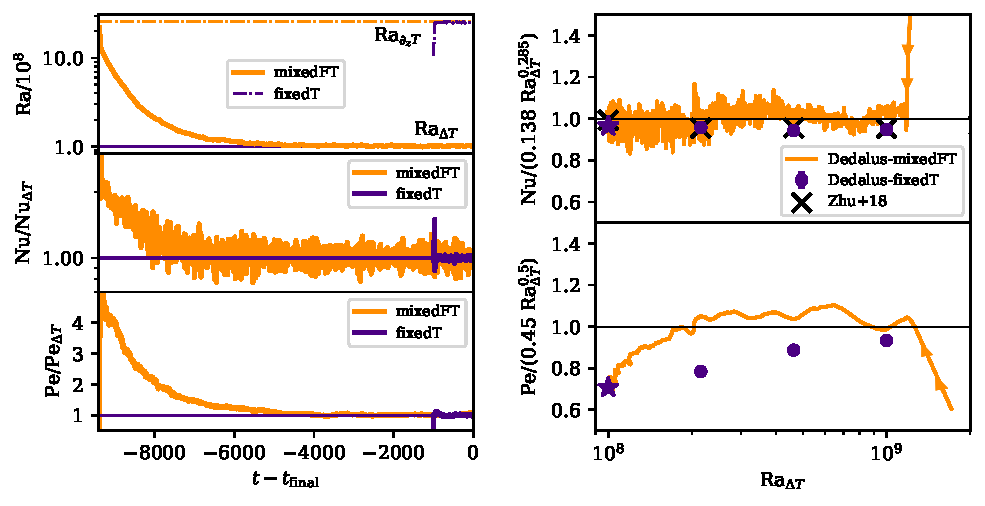
\includegraphics[width=\textwidth]{./figs/rbc_scalar_comparisons.pdf}
\caption{ 
\label{fig:rbc_scalar_comparisons} }
\end{figure}

In the left panels of Fig.~\ref{fig:rbc_scalar_comparisons}, we compare the time evolution of a mixed-FT (green) case to a fixed-T (orange) simulation.
In the top-left panel, we show the evolution of both the temperature and flux Rayleigh numbers of both simulations.
We show the input (flux) Ra of the mixed-FT case and the input (temp) Ra of the fixed-T case as horizontal lines, and overplot the evolution of the Ra$_{\Delta T}$ for the mixed-FT case and the evolution of Ra$_{\partial_z T}$ for the fixed-T case.
While the fixed-T case's flux Ra rapidly latches onto its final value, the mixed-FT case's temp Ra takes thousands of freefall times to equilibrate to its final value.
This fast evolution (fixed-T) and slow evolution (mixed-FT) is also seen in the equilibration of the Nusselt number (middle panel) and Peclet number (bottom panel).

A naive estimate of the thermal evolution timescale of these system is $t_{\text{therm}} = \sqrt{\Peff} = \sqrt{\text{Ra Pr}}$ \cite{anders&all2018}.
For the mixed-FT simulation presented here with Ra = 2.61 $\times 10^9$, this prediction returns $t_{\text{therm}} \approx 5\times 10^{4}$.
**I need to do a derivation and think about this more.

In the upper right panel of Fig.~\ref{fig:rbc_scalar_comparisons}, we show a plot of Nu vs Ra.
The green line shows the path through this space that our mixed-FT simulation traces out.
For reference, we show values of Nu reported for various fixed-T runs from previous work and from our own simulations conducted here.
Remarkably, the mixed-FT case seems to reliably perform a sweep through this parameter space.
However, despite seemingly tracing out the ``proper'' values of Nu(t) vs. Ra(t), the same is not true of the Reynolds number.
In the lower right panel, we plot the trace of Re vs Ra, and see that the mixed-FT case achieves a high value of Re compared to fixed-T cases as it sweeps toward lower values of Ra.
This makes sense; the mixed-FT simulation experiences a vigorous injection of kinetic energy during the convective transient and must slowly wind down from this energized state over time.
These traces through parameter space demonstrate that, unless measurements are taken after convergence is achieved, the dynamics sampled in a mixed-FT case may be misleading.

\begin{figure}
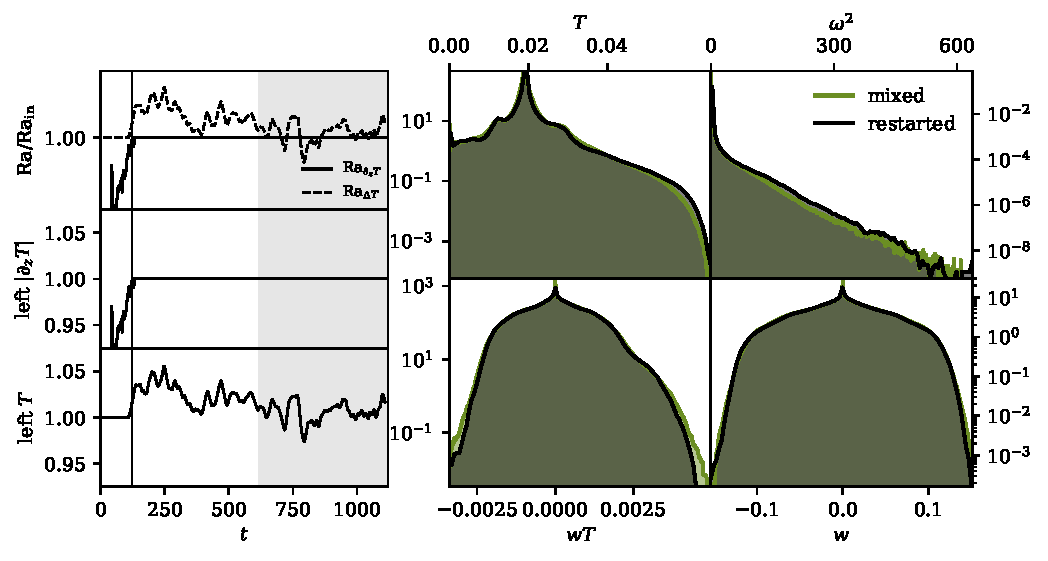
\includegraphics[width=\textwidth]{./figs/rbc_restart_description.pdf}
\caption{ 
\label{fig:rbc_restart_description} }
\end{figure}

The evidence displayed in Fig.~\ref{fig:rbc_scalar_comparisons} suggests that, in a volume-averaged sense, there is a comparable fixedT experiment for each mixedFT experiment.
This suggests that one can take advantage of the fast evolution on display in fixedT simulations to achieve rapidly equilibrated mixedFT simulations.
This is fortunate, as the rundown in mixedFT simulations is very costly:  not only do the turbulent dynamics at the large initial Rayleigh number need to be resolved (requiring more spectral modes to run the simulation), but thousands of freefall times must pass before convergence.
For a sense of scale, the first thousand freefall time units of the mixedFT case displayed in Fig.~\ref{fig:rbc_scalar_comparisons} took $1.43\times10^6$ iterations, or roughly $3.3 \times 10^4$ cpu-hours.
For comparison, the same time evolution (essentially the whole simulation) for fixedT boundary conditions took  $8.4\times10^5$ iterations, or roughly $5.4\times 10^3$ cpu-hours.
After these thousand freefall time units, the fixedT simulation has spent hundreds of freefall times in a statistically stationary state, whereas the mixedFT system continues to evolve towards its equilibrium state for an additional few thousands of time units.
This means that at these modest Rayleigh numbers (Ra$_{\Delta T} = 10^8$), the cost of equilibration of a mixedFT simulation is more than an order of magnitude larger than a fixedT simulation.

We take advantage of the fast evolution of fixedT simulations to achieve equilibrated mixedFT simulations by switching the boundary conditions on an equilibrated fixedT run.
Our procedure for achieving converged mixedFT dynamics using fixedT simulations is simple and takes place over these steps:
\begin{enumerate}
\item Run a fixedT simulation from convective transient to its statistically stationary state. 
Measure $\angles{\text{Nu}}$ in that state.
\item Re-nondimensionalize from a fixed temperature at the boundaries to a fixed flux.
This will involve setting the input Rayleigh number to a flux Ra, or $\text{Ra}_{\text{in}} = \angles{\text{Nu}}\text{Ra}_{\Delta T}$.
In our freefall nondimensionalization, this means setting the velocities in the mixedFT simulation to $\bm{u}_{\text{FT}} = \bm{u}_{\text{T}} / \sqrt{\angles{\text{Nu}}}$, and setting the temperature field to $T_{\text{FT}} = T_{\text{T}} / \angles{\text{Nu}}$.
\item Restart the simulation with mixedFT boundaries and continue timestepping.
\end{enumerate}

In the left panels of Fig. \ref{fig:rbc_restart_description}, we show that this procedure indeed seems to work.
We ran a simulation at Ra$_{\Delta T} = 10^8$, which has been reported to have $\text{Nu} \approx 26.1$ \cite{zhu&all2018}.
We restarted this simulation using mixedFT boundaries after roughly one thousand time units at an input value of Ra$_{\partial_z T} = 2.61 \times 10^9$.
Rolling averages of Ra$_{\Delta T} / 10^8$ and Ra$_{\partial_z T} / (2.61 \times 10^9)$ are shown through the full simulation.
As can been seen in the lower and bottom left panels, at the beginning of the simulation when fixedT boundary conditions are used, the flux at the lower boundary fluctuates but the temperature is precisely constant.
When these boundaries are switched for mixedFT boundaries, the left flux holds steady but the temperature is able to fluctuate.
Unlike in the mixedFT case displayed in Fig.~\ref{fig:rbc_scalar_comparisons}, there is no long thermal rundown in the mixedFT state, as the thermal profile has been equilibrated by the early fixedT portion of the run.

In order to verify if this restarting procedure achieves the same dynamics as a long rundown, we compare probability distribution functions of various quantities in our convective domains.
We display these PDFs in the right four panels of Fig.~\ref{fig:rbc_restart_description}.
We show the probability distributions of the temperature field (upper left), the enstrophy (upper right), the convective enthalpy flux (lower left), and the vertical velocity (lower right).
Visually, these PDFs are essentially identical, with perhaps small variations in their tails due to random extreme events which occur in one simulation but not the other.
The means, standard deviations, skewness, and kurtosis of each PDF is displayed in Table~\ref{table:pdf_values}, and the agreement is quite good.

\begin{table}[ht]
\caption{
}
\setlength{\tabcolsep}{12pt}
\label{table:speed}
\begin{center}
\begin{tabularx}{\textwidth}{c c c c c c}
\hline																	
Quantity &	Case	&	$\mu$	&	$\sigma$	&	Skewness	&	Kurtosis \\
%\hline \hline \multicolumn{6}{c}{\vspace{-0.2cm}}\\
%\multicolumn{6}{c}{\vspace{0.1cm}2D Runs} \\
\hline
$T$				&	mixedFT		&		$1.9 \times 10^{-2}$	&	$4.3 \times 10^{-3}$	&	1.1		&	15 \\
				&	mixedFT,r	&		$1.9 \times 10^{-2}$	&	$4.3 \times 10^{-3}$	&	1.3		&	17 \\
\hline
$\omega^2$		&	mixedFT		&		$1.3$					&	$6.4$					&	19		&	$5.2 \times 10^2$ \\
				&	mixedFT,r	&		$1.5$					&	$6.9$					&	18		&	$5.0 \times 10^2$ \\
\hline
$wT$			&	mixedFT		&		$1.9 \times 10^{-5}$	&	$9.4 \times 10^{-4}$	&	0.16	&	$3.1$ \\
				&	mixedFT,r	&		$1.9 \times 10^{-5}$	&	$9.3 \times 10^{-4}$	&	0.18	&	$3.2$ \\
\hline
$wT$			&	mixedFT		&		$7.9 \times 10^{-7}$	&	$4.9 \times 10^{-2}$	&	0.016	&	$2.7$ \\
				&	mixedFT,r	&		$-1.0 \times 10^{-6}$	&	$4.8 \times 10^{-2}$	&	0.02	&	$2.8$ \\
\hline																	
\end{tabularx}
\end{center}
\end{table}

The successful degree with which this mechanism reproduces the evolved dynamics suggests that thermal relaxation occurs in two parts:
\begin{enumerate}
\item Changes to the experimental energy reservoir, and
\item Restratification of the experiment.
\end{enumerate}
Through the use of complicated clever techniques \cite{anders&all2018} or simply through the choice of ``smart'' boundary conditions, the first of these pieces of thermal relaxation can be skipped.
For \RB convection with no-slip boundaries at the top and bottom plate, the latter part of thermal relaxation seems to be unimportant.
When complications such as stable layers are included in the model, we do not generally expect the latter piece of restratification to be completely insignificant, but for the simple case studied here it seems to be.

\subsection{Asymmetries induced by mixed boundaries}
\label{sec:asymmetries}
Now that we have verified a mechanism for rapidly and self-consistently achieving thermally equilibrated mixed-FT simulations, we study highly turbulent convection with mixedFT boundaries in an effort to understand the nature of asymmetries introduced to the problem by these boundary conditions.


\begin{figure}
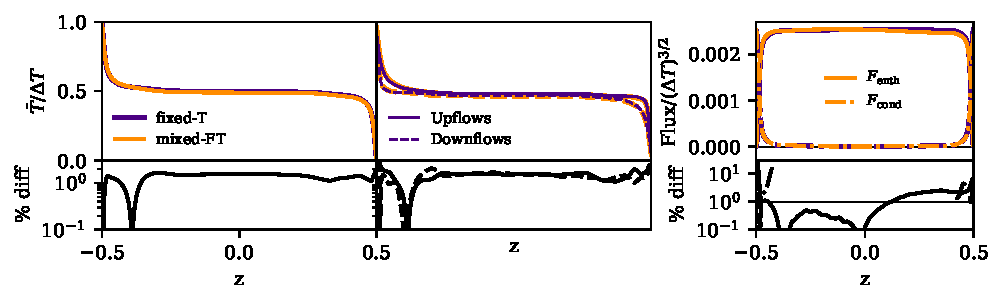
\includegraphics[width=\textwidth]{./figs/rbc_1D_profiles.pdf}
\caption{ 
\label{fig:rbc_1D_profiles} }
\end{figure}

In Fig.~\ref{fig:rbc_1D_profiles}, we compare the horizontally averaged, vertical profiles of our fixed-T and mixed-FT cases.
In the upper left panel, we show the mean temperature profiles achieved in the evolved state of both simulations.
Throughout the full depth, these profiles differ by less than 2\%, as shown in the lower left panel.
In the upper middle panel, we show the mean temperature profile in downflow areas compared to the mean temperature profile achieved in upflow areas.
Surprisingly, despite symmetrical boundary conditiosn in fixed-T simulations and asymmetrical boundary conditions in mixed-FT cases, we find precisely the same asymmetries in upflows/downflows for both sets of boundary conditions.
In general, we find that the boundary layer in upflows is more gradual in hot plumes, and the same is true for downflows and cold plumes.
Once again, these profiles agree to within < 2\%.

In the upper right panel of Fig.~\ref{fig:rbc_1D_profiles}, we plot the system fluxes for both cases.
the fluxes show very good agreement just like the temperature profile.
Throughout the bulk of the domain, the convective enthalpy fluxes agree to within a few \% or less (solid line in bottom right panel).
Due to the conductive fluxes approaching zero in the interior, we cannot measure a \% difference for this flux in the bulk, but we find that it is again within a few percent in the boudnary layers.

\begin{figure}
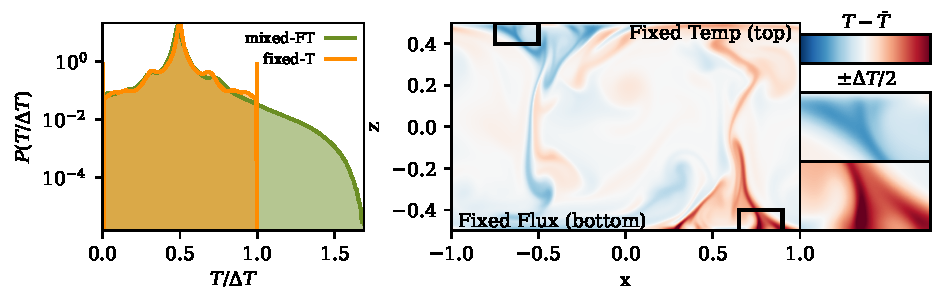
\includegraphics[width=\textwidth]{./figs/rbc_dynamics_asymmetries.pdf}
\caption{ 
\label{fig:rbc_dynamics_asymmetries} }
\end{figure}

In Fig.~\ref{fig:rbc_dynamics_asymmetries}, we examine the dynamical nature of the asymmetries which mixed-FT boundaries introduce into the simulation.
In the left panel, we plot the probability distribution functions of temperature measurements taken throughout the full domain.
These PDFs agree remarkably well for cold temperature (near the shared fixed-T boundary) and through the mean, but diverge for hot temperatures (where the boundary conditions differ).
We find that the mixed-FT pdf has a much longer tail and is capable of achieving much hotter instantaneous temperature values than a fixed-T boundary can.
In order to understand how this is possible, we examine a snapshot of the full temperature field.
In the middle panel, we plot the temperature anomaly -- the temperature field with the mean vertical profile subtracted from it.
We have outlined a portion of a cold plume near the upper (fixed-T) boundary and a portion of a hot plume near the lower (fixed-flux) boundary, and these regions are magnified in the lower right panels.
The fixed-T upper boundary suppresses temperature anomaly at the upper boundary and regulates the temperature minima which can be achieved.
The fixed-flux lower boundary does no such suppression and allows for extreme temperature values to be achieved in the plume-launching area.

\subsection{Fixed-Temp simulations can be used to skip thermal relaxation}


\subsection{Rotating \RB Convection}
\label{sec:rotating_results}


%%%%%%%%%%%%
%%%%%%%%%%%
% CONCLUSION
%%%%%%%%%%%
%%%%%%%%%%%%

\section{Discussion \& Conclusions}
\label{sec:extensions}

\begin{acknowledgments}
EHA acknowledges that this work was supported by NASA Headquarters under the NASA Earth and Space Science Fellowship Program -- Grant 80NSSC18K1199.
This work was additionally supported by NASA LWS grant NNX16AC92G and by the National Science Foundation under grant No.~1616538. 
Computations were conducted with support by the NASA High End Computing (HEC) Program through the NASA  Advanced Supercomputing (NAS) Division at Ames Research Center on Pleiades with allocation GID s1647.
\end{acknowledgments}


\bibliography{biblio.bib}

\appendix
\section{Table of Simulations}


\begin{table}[ht]
\caption{
}
\setlength{\tabcolsep}{12pt}
\label{table:speed}
\begin{center}
\begin{tabularx}{\textwidth}{c c c c c c c c c}
\hline																	
BCs	&	Ra	&	Pr	&	Ek	&	nz$\times$nx$\times$ny	&	cpu-hours &	Nu	&	Nu comp	&	Re \\
%\hline \hline \multicolumn{6}{c}{\vspace{-0.2cm}}\\
%\multicolumn{6}{c}{\vspace{0.1cm}2D Runs} \\
\hline
fixedT	&	$1.00 \times 10^8$	&	1	&	$\infty$	&	512x1024	&	$5.57 \times 10^3$	&	$25.4 \pm 0.1$	&	26.1	&	$3.18 \times 10^3$ \\
mixedFT	&	$2.61 \times 10^9$	&	1	&	$\infty$	&	1024x2048	&	$1.21 \times 10^5$	&	$25.3 \pm 0.2$	&	26.1	&	$3.31 \times 10^3$ \\
fixedT	&	$2.15 \times 10^8$	&	1	&	$\infty$	&	512x1024	&	$5.73 \times 10^3$	&	$31.3 \pm 0.2$	&	31.2	&	$5.17 \times 10^3$ \\
fixedT	&	$4.64 \times 10^8$	&	1	&	$\infty$	&	1024x2048	&	$4.66 \times 10^4$	&	$38.4 \pm 0.3$	&	38.9	&	$8.60 \times 10^3$ \\
fixedT	&	$1.00 \times 10^9$	&	1	&	$\infty$	&	1024x2048	&	$5.58 \times 10^4$	&	$48.0 \pm 0.4$	&	48.3	&	$1.33 \times 10^4$ \\
fixedT	&	$2.15 \times 10^9$	&	1	&	$\infty$	&	1024x2048	&	$6.38 \times 10^4$	&	$60.4 \pm 0.5$	&	61.1	&	$1.99 \times 10^4$ \\
\hline																	
\end{tabularx}
\end{center}
\end{table}



\end{document}
